\section{Results}
\subsection{Testing StabilityFinder: The Gardner toggle switch}

This toggle switch model was developed by T.~S. Gardner~\autocite{Gardner:2000vha}. This model consists of two mutually repressing transcription factors and is defined by the following ODEs:

\begin{align}
\frac{du}{dt} &= \frac{a_1}{1+v^{\beta}} - u \label{eq:gard_1} \\
\frac{dv}{dt} &= \frac{a_2}{1+u^{\gamma }} - v\label{eq:gard_2}
\end{align}
Where $a_1$ and $a_2$ are the effective rates of synthesis of repressors 1 and 2 respectively. \textit{u} is the concentration of repressor 1 and \textit{v} the concentration of repressor 2. \textit{$\beta$} is the cooperativity of repression of promoter 1 and \textit{$\gamma$} of repressor 2. In their paper,  T.~S. Gardner~\autocite{Gardner:2000vha} state that there are two conditions for bistability of this toggle switch model. That $a_1$ and $a_2$ are balanced and that $\beta$ and $\gamma$ are \textgreater 1. In order to test our methodology, we used StabilityFinder to find the posterior distribution for which this model exhibits bistable behaviour. So setting the desired behaviour to bistable, and using for priors a wide range of values that includes the values used in the Gardner paper, we test StabilityFinder to see if it finds the same conditions as the ones set by T.~S. Gardner. The prior distributions used are shown in Table~\ref{tab:gard}. The posterior distribution calculated by StabilityFinder is shown in Figure~\ref{fig:Gard_post}.

\cleardoublepage
\begin{figure}[t]
\centering
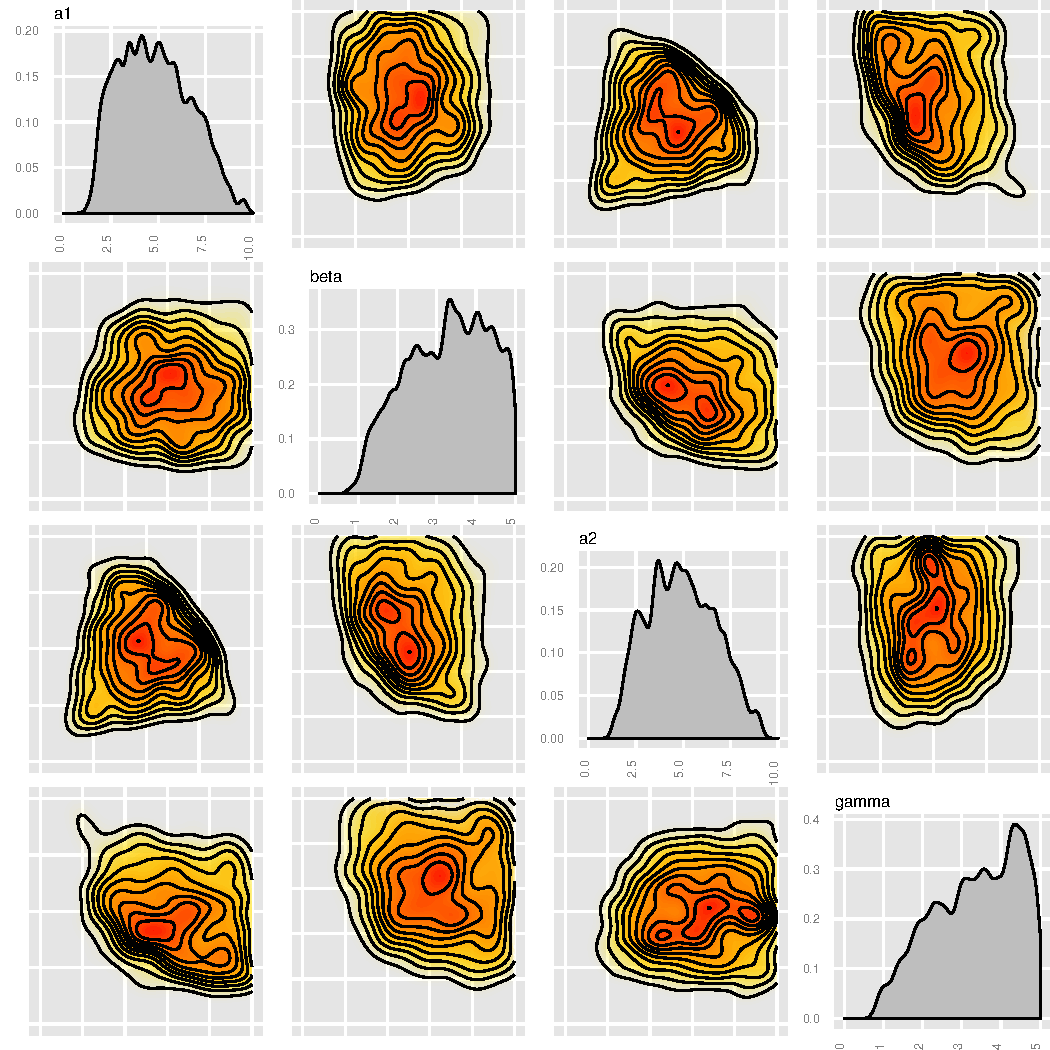
\includegraphics[scale=0.7]{chapterModelling/images/Gardner/posterior.pdf}
\caption[The posterior distribution of the bistable Gardner toggle switch]{The posterior distribution of the bistable Gardner toggle switch. The parameters $a_1$, $a_2$ represent to the effective synthesis rate of repressors 1 and 2 respectively. Parameters $\beta$, $\gamma$ represent the cooperativity on repressors 1 and 2 respectively. The marginal distributions of each parameter are found on the diagonal and pairwise joint distributions along the sides.}
\label{fig:Gard_post}
\end{figure}


\begin{figure}[t]
\centering
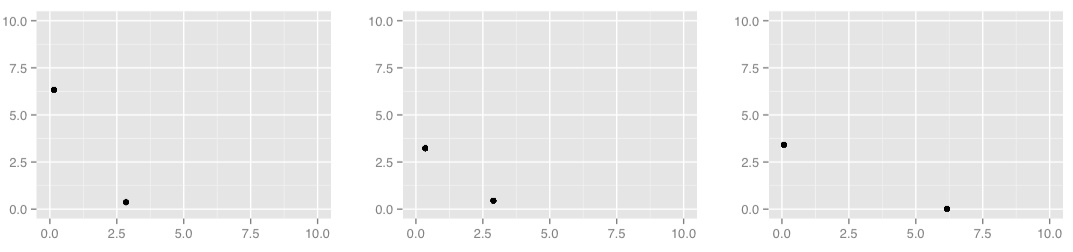
\includegraphics[scale=0.3]{chapterModelling/images/Gardner/phase_plots.png}
\caption{A sample of the phase plots produced from the final population of the Gardner switch.}
\label{fig:det_gard_phase}
\end{figure}

\begin{table}[b]
\centering
\caption{Gardner switch priors}
\label{tab:gard}
\begin{tabular}{cccc|cc}
\multicolumn{4}{c|}{Parameters} & \multicolumn{2}{c}{Species} \\ %\hline
$a_1$   & $\beta$   & $a_2$   & $\gamma$  &   $s_1$      &       $s_2$   \\
0-10    & 0-5       & 0-10    &  0-5      &      0-100   &          0-100   
\end{tabular}
\end{table}

These results agree with the results reported by the original paper~\autocite{Gardner:2000vha} . For this switch to be bistable $a_1$ and $a_2$ must be balanced while $\beta$ and $\gamma$ must both be \textgreater 1, as can be seen in the marginal distributions of $\beta$ and $\gamma$ in Figure~\ref{fig:Gard_post}. The conditions set by the original paper for parameters $a_1$ and $a_2$ are met, as the joint distribution shown in Figure~\ref{fig:Gard_post} matches the bifurcation lines calculated in the original paper. 
This successful test demonstrates that StabilityFinder can be used to find the stability a model is capable of as well as the parameter ranges that can produce that. This allows us to confidently apply the methodology to further models.
%-%-%-%-%-%-%%-%-%-%-%-%-%%-%-%-%-%-%-%

\subsubsection{Comparing the deterministic and stochastic cases} 
    
There are two main ways of modelling a system, deterministically and stochastically. Deterministic modelling utilises ordinary differential equations (ODE) and models the concentrations of the species (proteins or other molecules) by time-dependent variables~\autocite{deJong:2002ft}. Rate equations are used to model gene regulation where the rate of production of a species is a function of the concentrations of the other species~\autocite{deJong:2002ft}. When modelling deterministically the model is viewed as a system which, with sufficient knowledge of the system, its behaviour is entirely predictable. Nevertheless we are still a long way away from having complete knowledge of a system of interesting size~\autocite{wilkinson:2006}. Deterministic modelling also assumes a homogenous mixture where species concentrations vary continuously and deterministically, assumptions that often are not met \textit{in vivo}. A cell is spatially and temporally separated, due to small molecule numbers and fluctuations in the timing of processes~\autocite{deJong:2002ft}.  
   
In stochastic modelling, species are measured in discrete amounts rather than concentrations and a joint probability distribution is used to express the probability that at time \textit{t} the cell contains a number of molecules of each species~\autocite{deJong:2002ft}. It takes uncertainty into account and is thus often more appropriate for modelling cellular systems, although more computationally intensive. In stochastic systems the Gillespie algorithm is widely used to simulate the time-evolution of the state of the system~\autocite{Warren:2005kea}.

The toggle switch has been modelled both deterministically and stochastically, with the two methods producing different results. Thus here we use StabilityFinder to compare the stabilities that the model is capable of, under the different simulation types. By using the same framework, and the same prior distributions for the models, one can directly compare the posterior distributions produced by the deterministic and the stochastic case, and uncover the effects that are due to the stochasticity of the system. This is relevant in a a biological model in which small molecule numbers and external noise are not negligible. Using StabilityFinder and using the same priors for the two models (Table~\ref{tab:gard_det_stoch}), we calculated the posterior for each both bistable models. The results are shown in Figure~\ref{fig:Gard_summary}. The prior ranges used are much wider than in the test case in order to allow more flexibility in both models and have a greater range over which to compare the models. 


\begin{table}[h]
\centering
\caption{Gardner switch priors in the deterministic and stochastic cases}
\label{tab:gard_det_stoch}
\begin{tabular}{cccc|cc}
\multicolumn{4}{c|}{Parameters} & \multicolumn{2}{c}{Species} \\ %\hline
$a_1$   & $\beta$   & $a_2$   & $\gamma$  &   $s_1$      &       $s_2$   \\
0-60    & 0-5       & 0-60    &  0-5      &      0-100   &          0-100   
\end{tabular}
\end{table}

\begin{figure}[p]
\centering
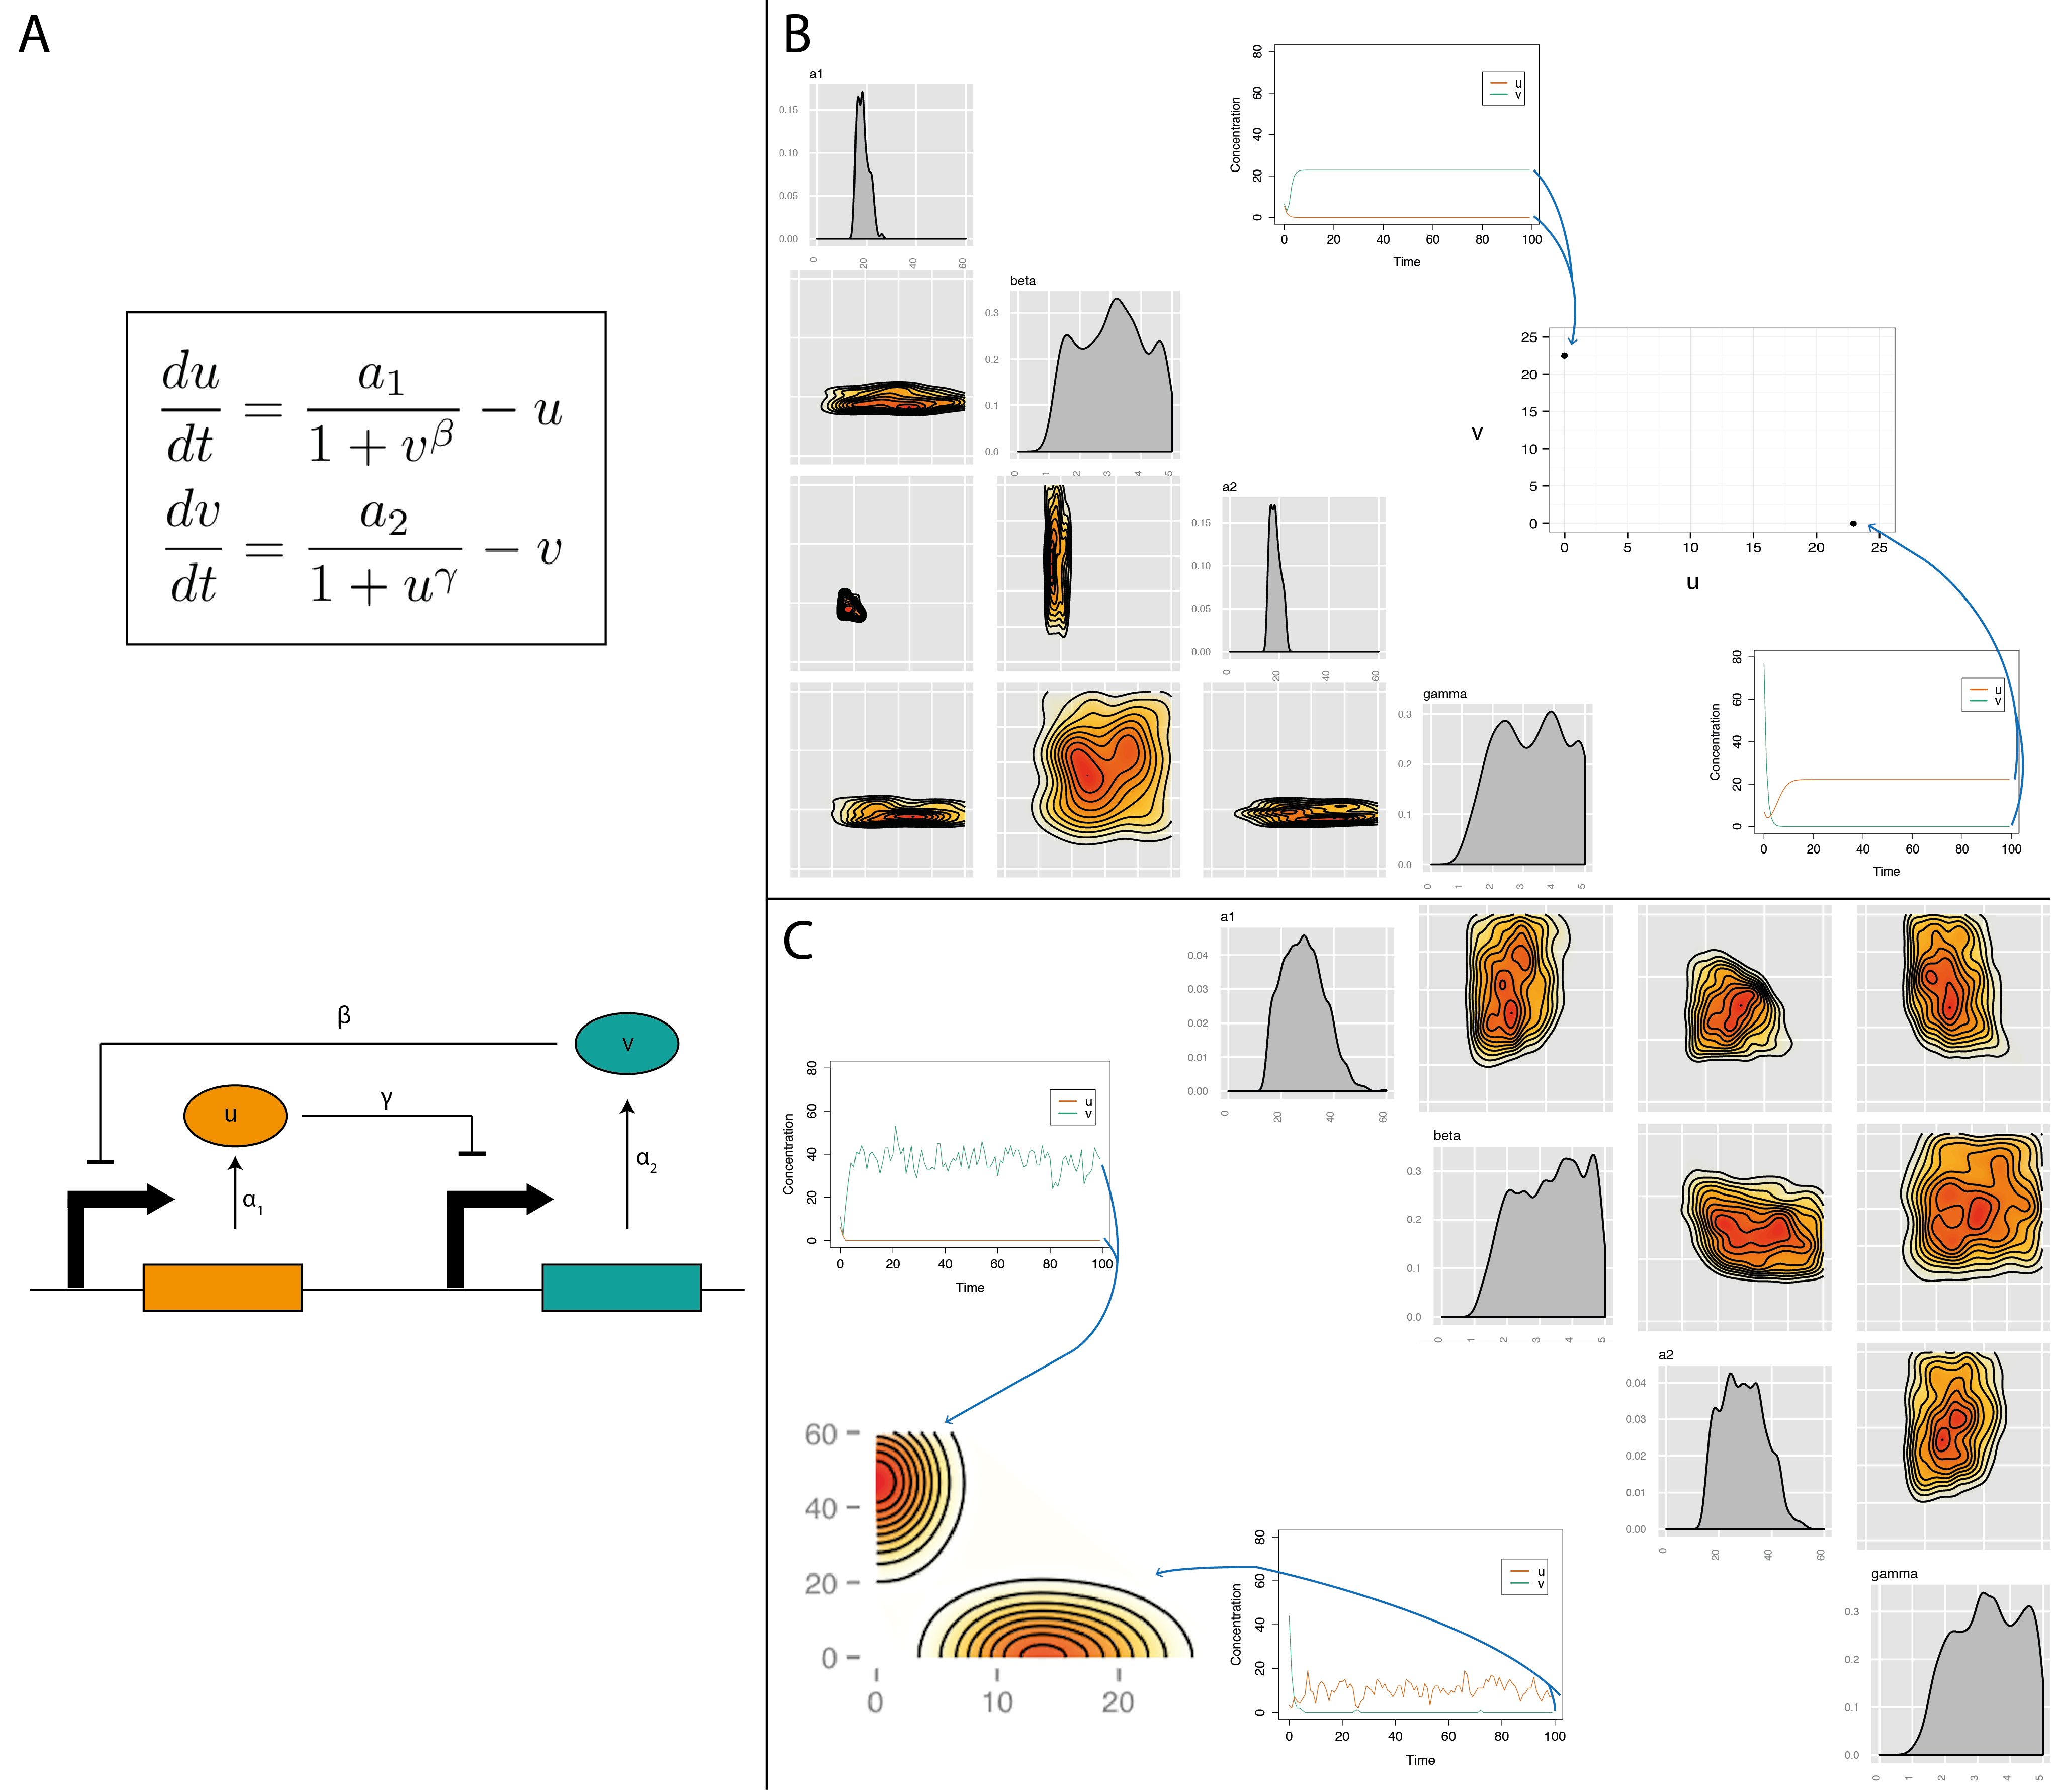
\includegraphics[scale=0.45]{chapterModelling/images/Gardner/summary.png}
\caption[The stochastic and deterministic cases of the Gardner toggle switch]{The Gardner toggle switch is modelled stochastically and deterministically. The model is shown graphically and mathematically in (A), The posterior and phase space of the deterministic model is shown in (B) and of the stochastic case in (C).}
\label{fig:Gard_summary}
\end{figure}


%\begin{figure}[p]
%\centering
%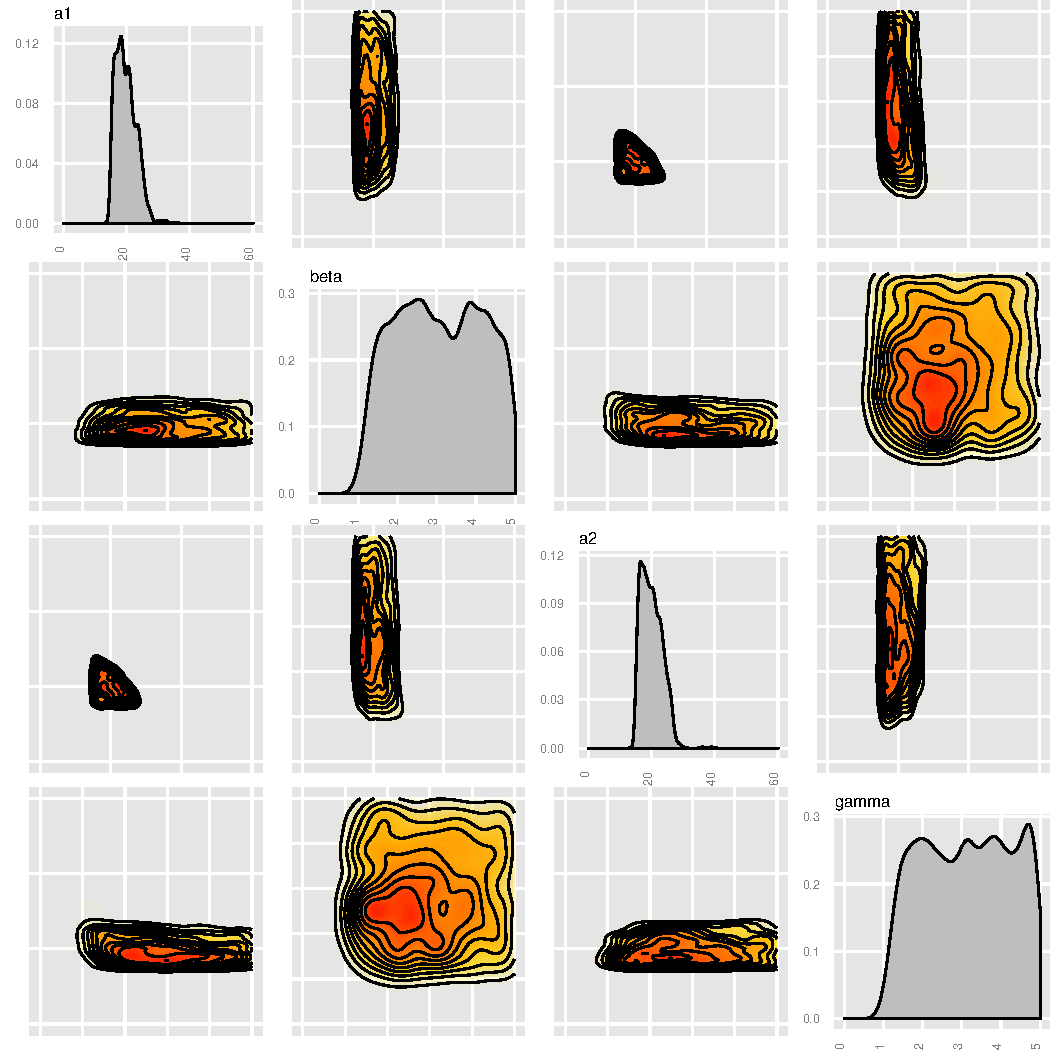
\includegraphics[scale=0.5]{chapterModelling/images/Gardner/wide_var/posterior_deter_high_mean.pdf}
%\caption{The posterior distribution of the deterministic model of the Gardner toggle switch.}
%\label{fig:Gard_post_det_high}
%\end{figure}
%
%\begin{figure}[p]
%\centering
%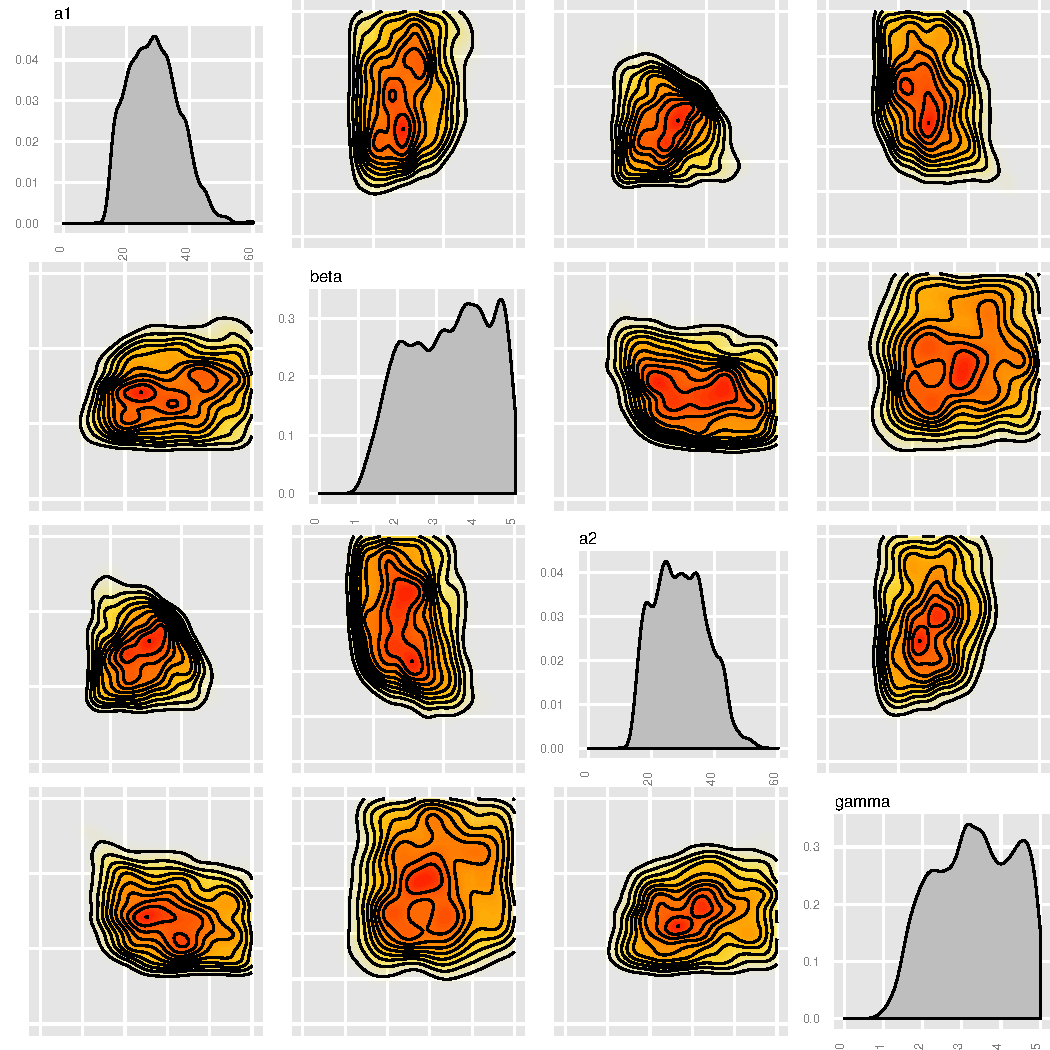
\includegraphics[scale=0.5]{chapterModelling/images/Gardner/wide_var/posterior_stch_high_mean.pdf}
%\caption{The posterior distribution of the stochastic model of the Gardner toggle switch.}
%\label{fig:Gard_post_stch}
%\end{figure}
\clearpage
As can be seen in the above results, stochasticity has a big effect on the posterior. Firstly, a greater parameter range can produce a bistable behaviour when stochastic effects are taken into account. The condition set by T.~S Gardner~\autocite{Gardner:2000vha} for the values of $a_1$ and $a_2$ to be balanced holds in both the deterministic and stochastic cases but in the stochastic case this is met by a wider range of values. The second conditions of $\beta$, $\gamma$ \textgreater 1 also needs to be met in the stochastic case. The posterior of the deterministic model shown in Figure~\ref{fig:Gard_summary}B, parameters $a_1$ and $a_2$ also have an upper limit of values they can take and still create a bistable switch. In order to test this result, we find the roots of the system for large values of  $a_1$ and $a_2$ in order to see if three roots are still found, two stable and one unstable. The results as shown in Figure indicate that the system is still bistable for increasing values of $a_1$ and $a_2$. This suggests that the upper limit found with StabilityFinder is an artefact of the variance limit imposed on the system. In order to find the steady states we impose an accepted distance from a given total variance for each model. When the two clusters of steady state values are too far removed, this increases total variance of the system and would consequently be rejected in StabilityFinder.

\begin{figure}[h]
\centering
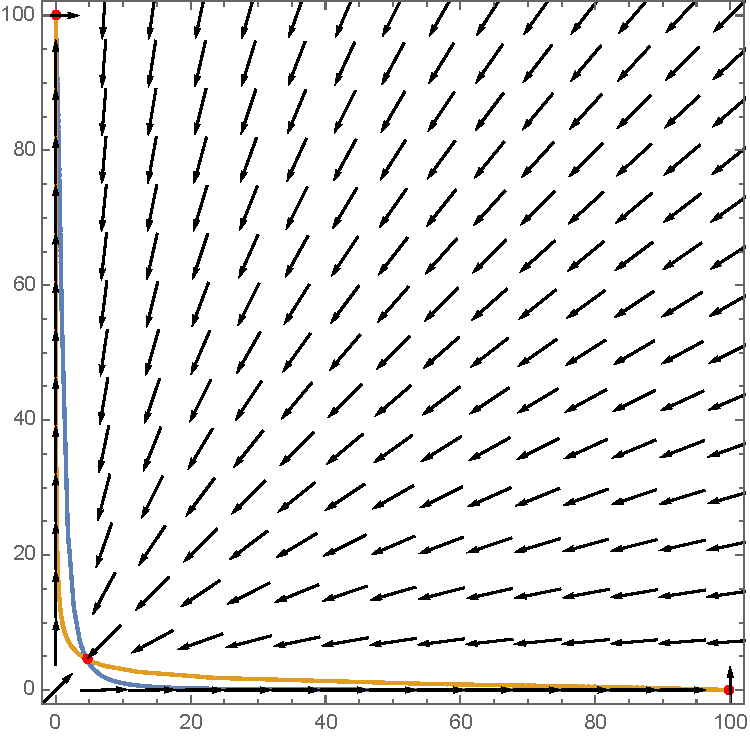
\includegraphics[scale=0.6]{chapterModelling/images/Gardner/gardner_solve_roots_a1a2_big.pdf}
\caption[Solving the Gardner toggle switch.]{Solving the Gardner toggle switch. The parameters values used are:  $a_1$, $a_2$ = 100 and $\beta$, $\gamma$ = 2. The system has three roots, of which one was found to be unstable and the other two stable. This result disagrees with that found in StabilityFinder, that $a_1$ and $a_2$ have an upper limit of 30.}
\label{fig:Gard_robst}
\end{figure}

 When stochasticity is taken into account, robustness increases significantly as seen in Figure~\ref{fig:Gard_robst}. This indicates that stochasticity increases the ability of the model to withstand fluctuations in parameter values and still produce the desired bistability. A deterministic model cannot predict this increased robustness.
 
\begin{figure}[h]
\centering
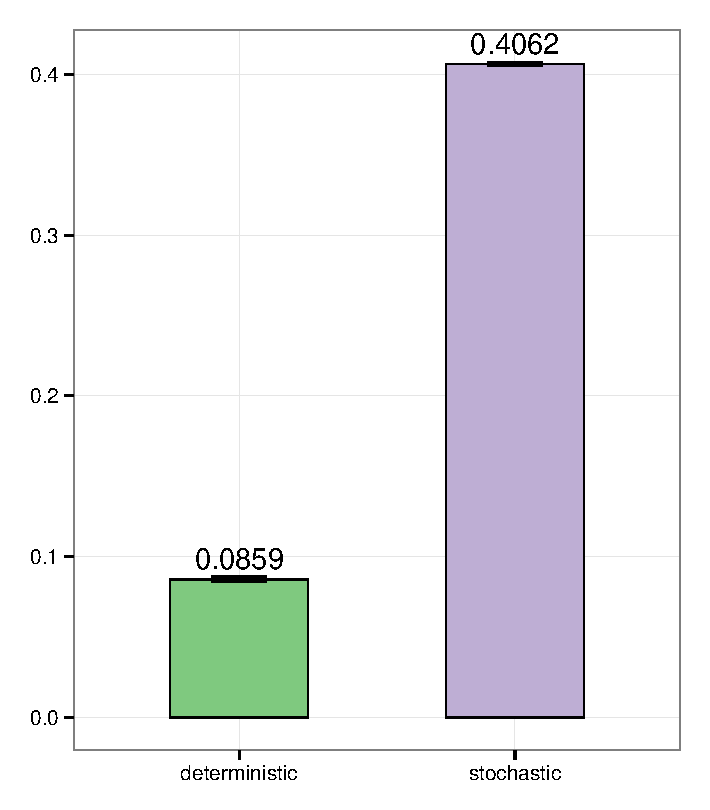
\includegraphics[scale=0.6]{chapterModelling/images/Gardner/wide_var/robustness_comparison.pdf}
\caption{Comparing the robustness of the deterministic and stochastic Gardner switch models}
\label{fig:Gard_robst}
\end{figure}



In order to check if this increase in robustness is caused by the different clustering methods used in the stochastic and deterministic cases, we tested the deterministic case by running the exact same model but using the clustering algorithm used in the stochastic case. Then we compared the robustness using the method outlined above. These results are shown in Figure~\ref{fig:Gard_det_stoch_kmeans}

\begin{figure}[h]
\centering
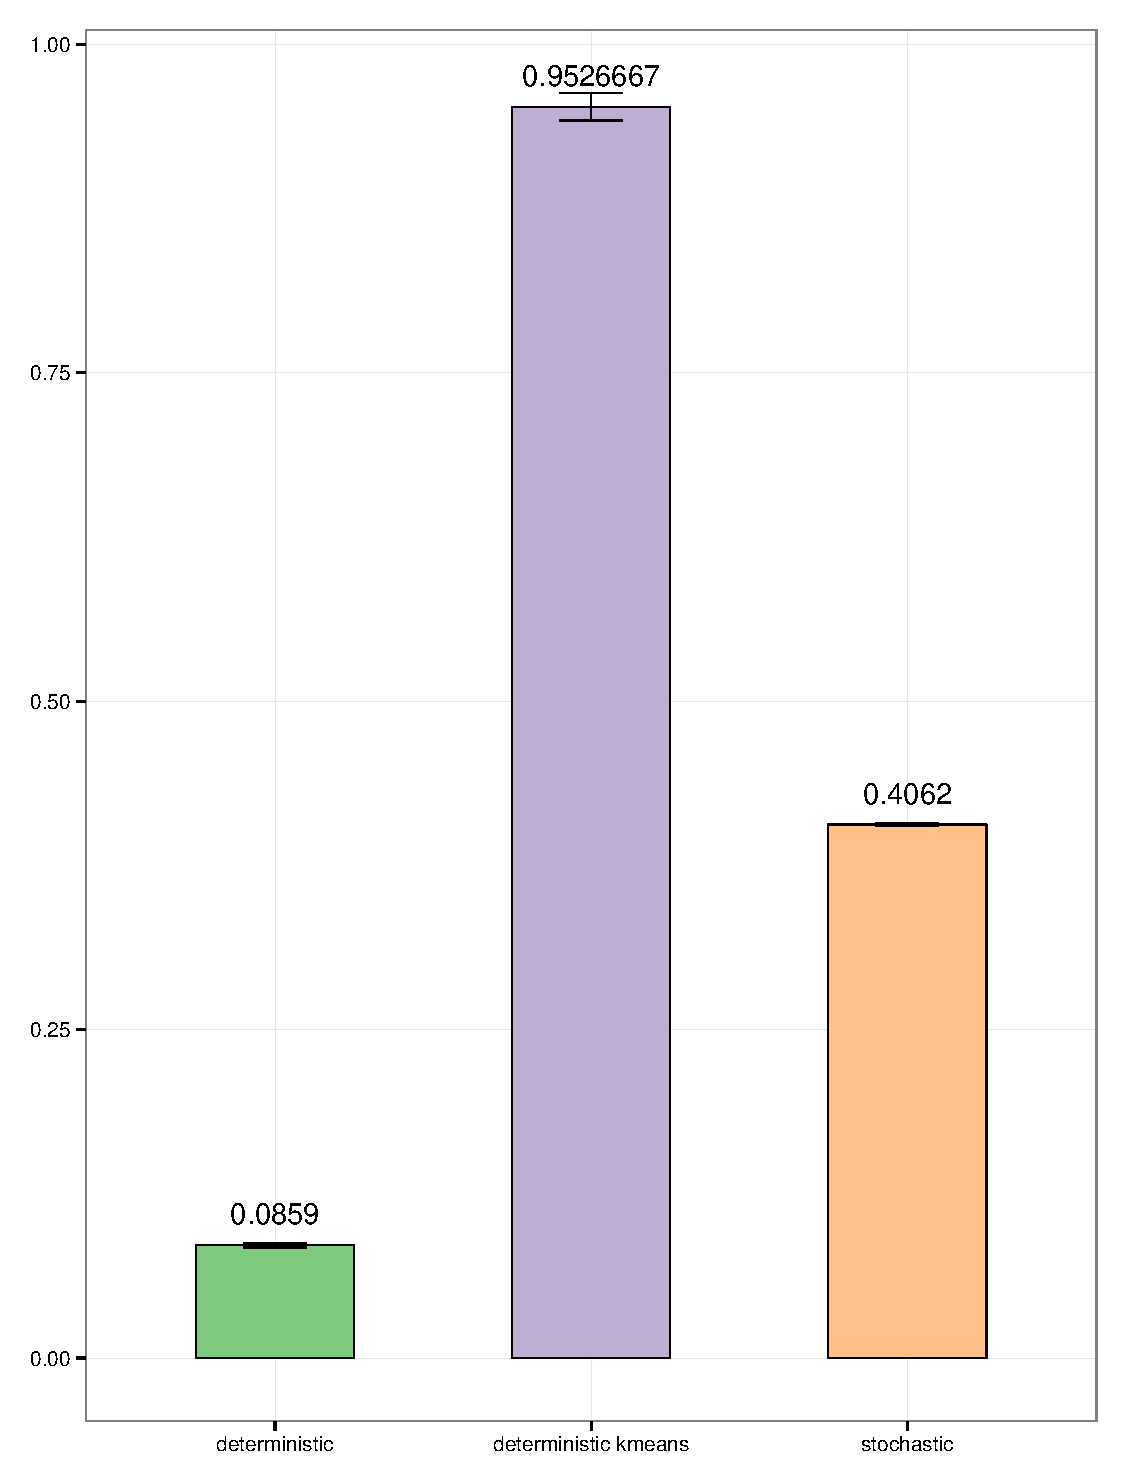
\includegraphics[scale=0.5]{chapterModelling/images/Gardner/robustness_comparison_gard_stoch_determ_kmeans.pdf}
\caption{The effect of the clustering methods on robustness measurements}
\label{fig:Gard_det_stoch_kmeans}
\end{figure}

This indicates that the clustering methods used have a big effect on the robustness measured. The increase in robustness seen in Figure~\ref{fig:Gard_robst} could be a bias of the clustering algorithms.
\clearpage
